\label{sec:THanetal}

Higgs pair production $pp\rightarrow hh$ offers a direct path to pin
down the Higgs self-coupling $\lambda$ at a hadron collider~\cite{Eboli:1987dy, Dicus:1987ic, Glover:183945, Plehn:1996wb, Djouadi:1999rca, Li:2013rra}.  
Theoretical studies as well as current analyses
point to the $b\bar{b}\gamma\gamma$ decay as the most promising
signature at the LHC~\cite{ATLAS-CONF-2016-004, Aad:2015xja}. 
For the high-luminosity LHC (HL-LHC),
ATLAS and CMS projections indicate a very modest sensitivity to the
Higgs self-coupling~\cite{ATL-PHYS-PUB-2017-001, CMS-PAS-FTR-16-002}. 
In the optimistic scenario that we can neglect systematic
uncertainties, those studies indicate that the LHC will probe the
coupling at 95\% confidence level $-0.8 < \kappa_\lambda < 7.7$, where the SM value is $\kappa_\lambda = \lambda/\lambda_{SM}=1$, 
falling short in precision in comparison to other Higgs 
property measurements at the LHC, and far from satisfactory in probing the
Higgs potential. For example, ${\cal O}(1)$ determination of $\kappa_\lambda$ would be required to 
test some of the EW Baryogenesis models~\cite{Kobakhidze:2015xlz, Chen:2017qcz, Gan:2017mcv, Cao:2017oez, Jain:2017sqm, deVries:2017ncy, Reichert:2017puo, Carena:2018vpt}.

Because of the rapidly growing gluon luminosity at higher energies,
the $hh$ production cross section increases by about a factor of
4~(40) at 27~(100)~\UTeV.  This means that at the HE-LHC with the
anticipated integrated luminosity of $15~\iab$ the number of events in
the $b\bar{b} \; \gamma \gamma$ channel increases by a factor $4
\times 5 = 20$ to around 5k events.  A 100~\UTeV hadron collider with
a projected integrated luminosity of $30~\iab$ features another
increase by a factor $10 \times 2=20$, to around 100k expected Higgs
pair events in the Standard Model.
This estimate shows how the combination of increased energy and
increased luminosity slowly turns Higgs pair production into a valid
channel for precision measurements~\cite{Goncalves:2018yva}. 

%%%%%%%%%%%%%%%%%%%%%%%%%%
\asubsubsubsection{Information in Distributions}

Previous studies have shown that multivariate analysis, taking into 
account kinematic distributions, gives a substantially better reach 
on the Higgs self coupling over the purely rate-based 
analysis~\cite{Goncalves:2018yva,Kling:2016lay,Barger:2014qva,Bauer:2017cov}. In the following, we therefore 
summarise which kinematic features include information about the 
Higgs self-coupling. 

At leading order, Higgs pair production receives contributions both 
from a triangular loop diagram sensitive to the Higgs-self coupling 
and from a box or continuum diagram. The box contribution completely 
dominates the total rate over most of the phase space, making the Higgs 
coupling measurements a challenge. While we can define a number of
kinematic observables describing the continuum backgrounds, the
measurement of the Higgs self-coupling relies on a simple $2 \to 2$
process with two independent kinematic variables.

Three distinct phase space regions provide valuable information on a
modified Higgs self-coupling, all from a large destructive interference 
between the triangle and box contributions. First, there is the 
threshold~\cite{Plehn:1996wb, Djouadi:1999rca, Li:2013rra, Baur:2002rb, Baur:2002qd,Li:2015yia} in the partonic centre of mass energy 
$ m_{hh} \approx 2 m_h$. Based on the effective
Higgs-gluon Lagrangian~\cite{Shifman:1979eb,  Kniehl:1995tn, Spira:2016zna} we can therefore write the
corresponding amplitude for Higgs pair production as
%
\begin{equation}
\frac{\alpha_s}{12 \pi v}
\left( \frac{\kappa_\lambda \lambda_\text{SM}}{s-m_h^2} - \frac{1}{v} \right) 
\to
\frac{\alpha_s}{12 \pi v^2}
\left( \kappa_\lambda -1 \right) \stackrel{\text{SM}}{=} 0 \; .
\label{eq:higgs_pair}
\end{equation}
%
While the heavy-top approximation is known to give a poor description
of the signal kinematics as a whole, it does describe the threshold
dependence correctly~\cite{Baur:2002rb, Baur:2002qd,Li:2015yia}. 
This indicates that we can search
for a deviation of the Higgs self-coupling by looking for an
enhancement of the rate at threshold. 
Second, an enhanced sensitivity to the self-coupling appears as top
mass effect. For large positive values of $\lambda$ absorptive imaginary 
parts lead to a significant dip in the combined rate at the threshold 
$m_{hh} \approx 2 m_t $~\cite{Dolan:2012rv, Barr:2013tda, Kling:2016lay}. 
The sharpest interference dip takes place near $\kappa_\lambda\approx 2$
while for negative values of $\kappa_\lambda$ the interference 
becomes constructive.
Finally, the triangular and box amplitudes have a generally different
scaling in the limit $m_{hh} \gg m_h, m_t$
~\cite{Plehn:1996wb, Djouadi:1999rca, Li:2013rra,Dolan:2012rv, Barr:2013tda}. While the triangle amplitude features an 
explicit suppression of either $m_h^2/m_{hh}^2$ or 
$m_t^2/m_{hh}^2$ at high invariant mass, the box diagrams drops 
more slowly towards the high-energy regime. This explains why a 
rate based analysis focusing on the high di-Higgs mass region
only has limited sensitivity. The impact of all three kinematic features can be quantified
statistically and  indicate that essentially the full
information on the Higgs self-coupling can be extracted through a
shape analysis of the $m_{hh}$ distribution~\cite{Bauer:2017cov}. 

In Fig.~\ref{fig:madmax_diff} we present the signal and background 
distributions for three relevant kinematic variables: $m_{hh}$, $p_{T,h}$
and $\Delta R_{\gamma\gamma}$. Using the \textsc{MadMax} 
approach~\cite{Cranmer:2006zs, Plehn:2013paa}, based on the Neyman Pearson Lemma we 
also estimate the maximum significance with which any multi-variate 
analysis will be able to extract an anomalous self-coupling 
$\kappa_\lambda \neq1$. The corresponding differential distribution of 
maximum significance are shown as solid lines in Fig.~\ref{fig:madmax_diff}. 
In addition to the signal features, the significance is limited by the rapidly dropping 
backgrounds, covering both of the above-mentioned regions with an enhanced dependence 
on the triangle diagram. In the absence of background, the significance 
indeed peaks between the production threshold and the top-mass
threshold~\cite{Kling:2016lay}.  The drop towards large values of $m_{hh}$
is a combination of the dominance of the box diagram in the signal and
the limited number of expected signal events.  The significance with
which we can extract modified self-couplings either smaller
($\kappa_\lambda = 0$) or larger ($\kappa_\lambda = 2$) than in the
Standard Model shows a similar phase space dependence. The only
difference is a slightly harder significance distributions for
$\kappa_\lambda = 2$, an effect of the dip at
$m_{hh}\approx 2m_t$.

%---------------------------------------------
\begin{figure*}[t]
  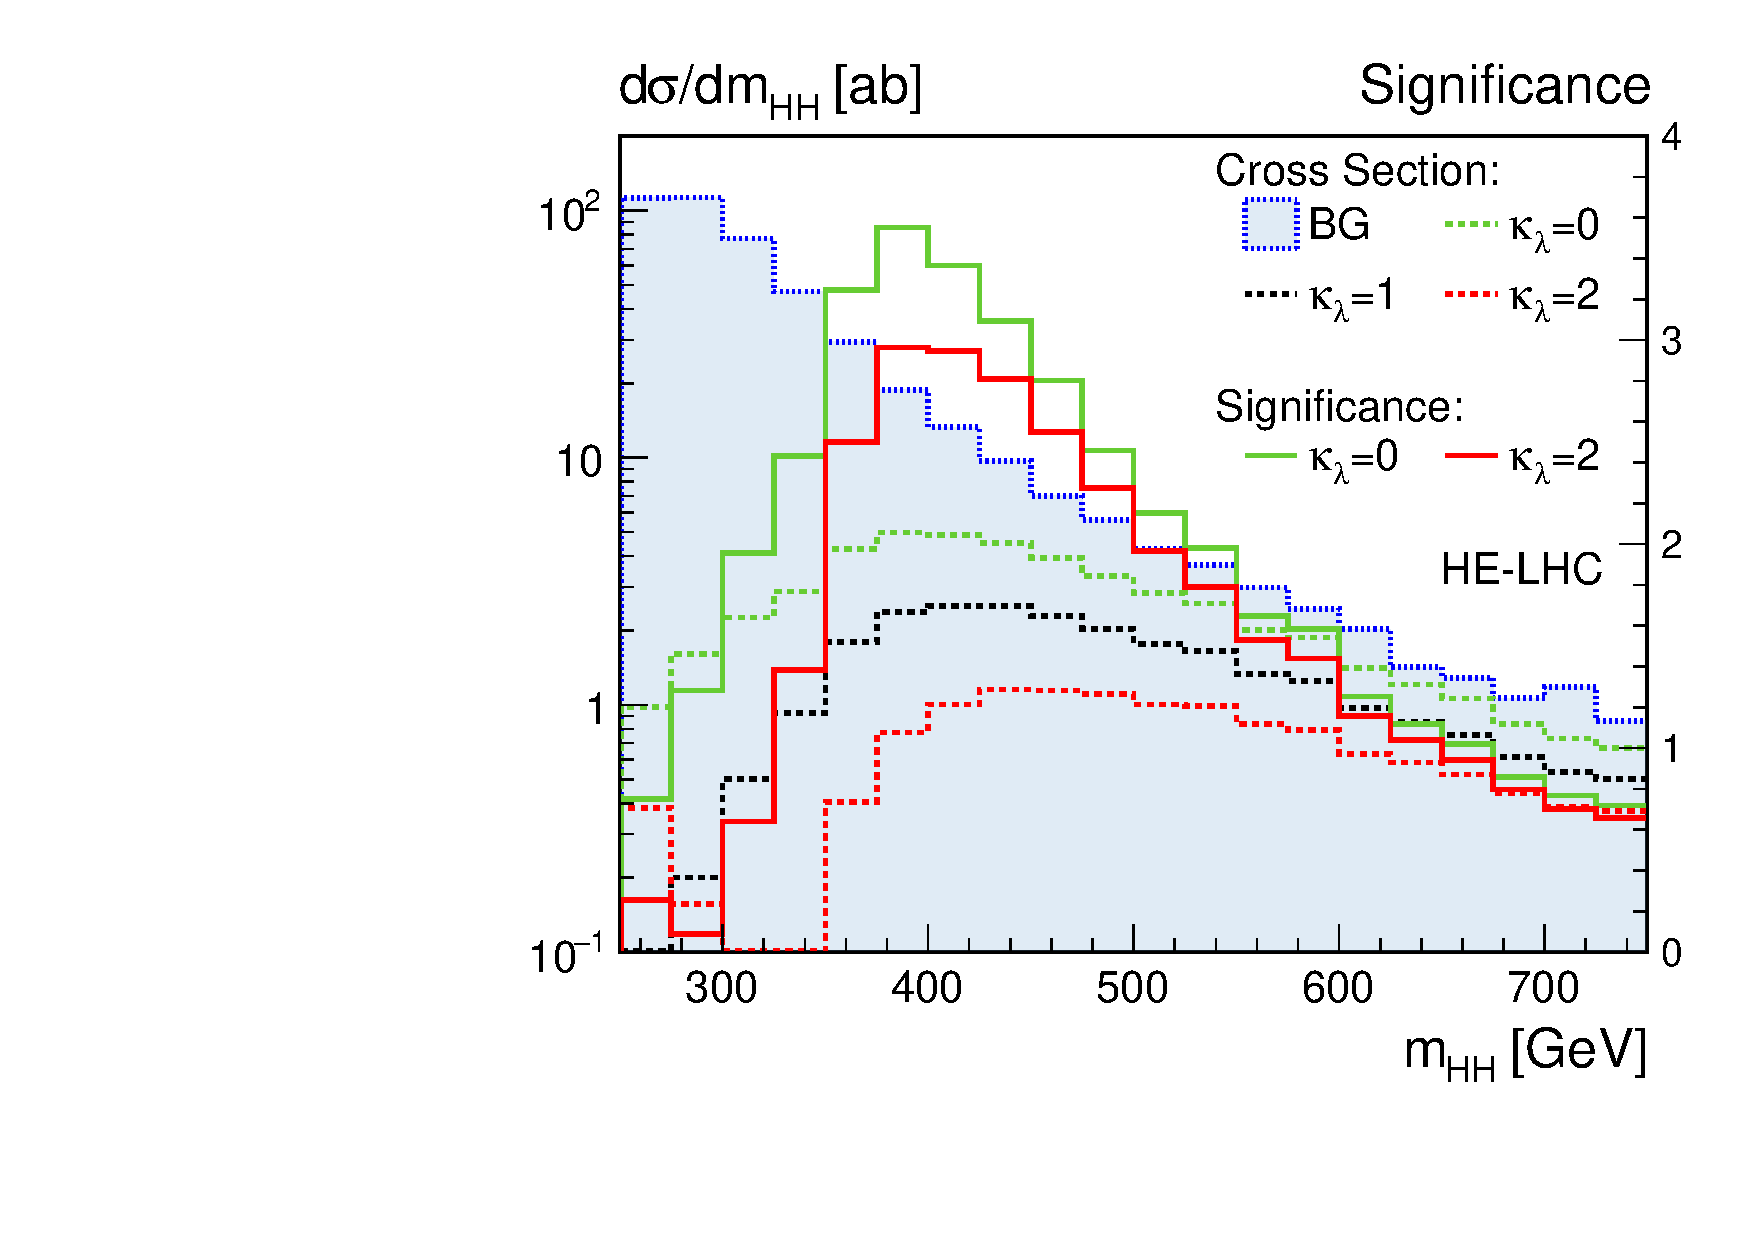
\includegraphics[width=0.32\textwidth]{\main/section3/plots/Plot_mhh_27TeV}
  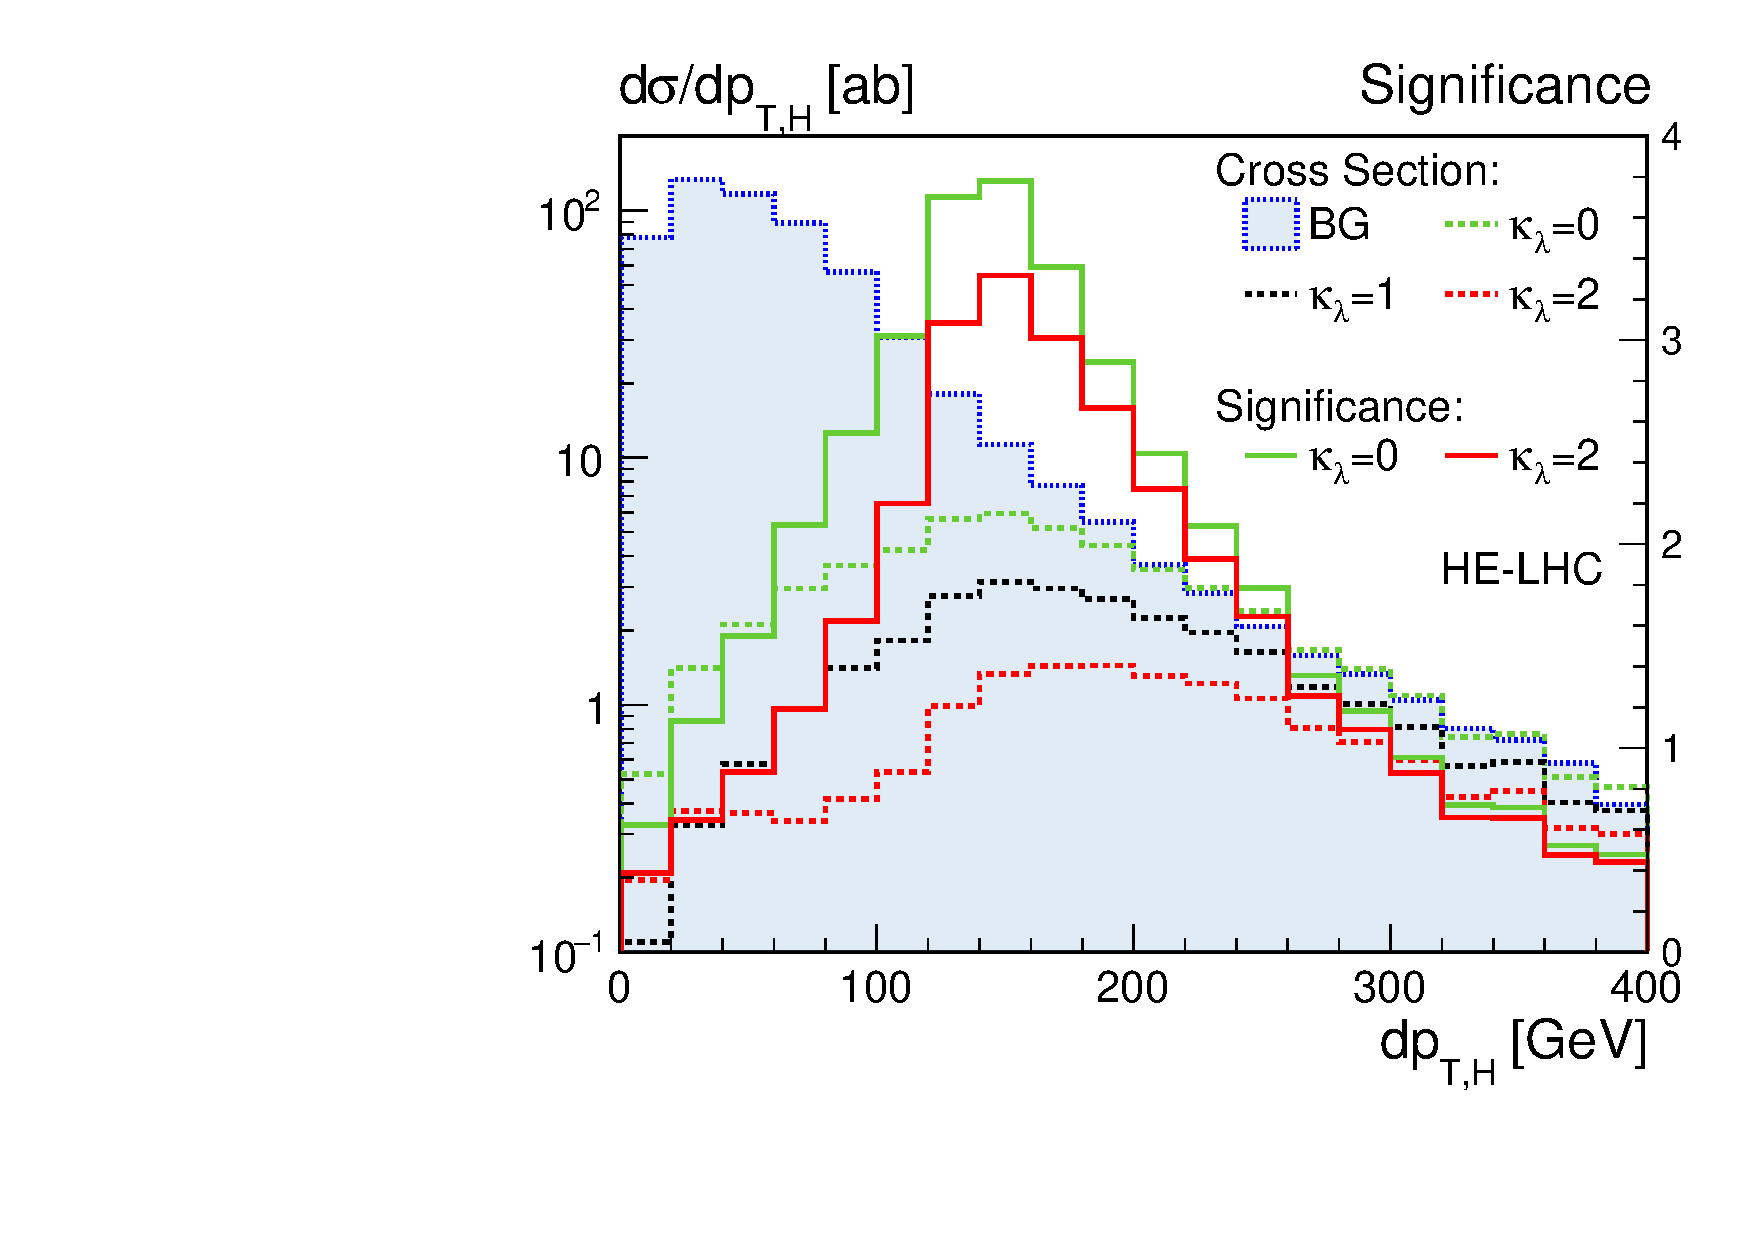
\includegraphics[width=0.32\textwidth]{\main/section3/plots/Plot_pth_27TeV}
  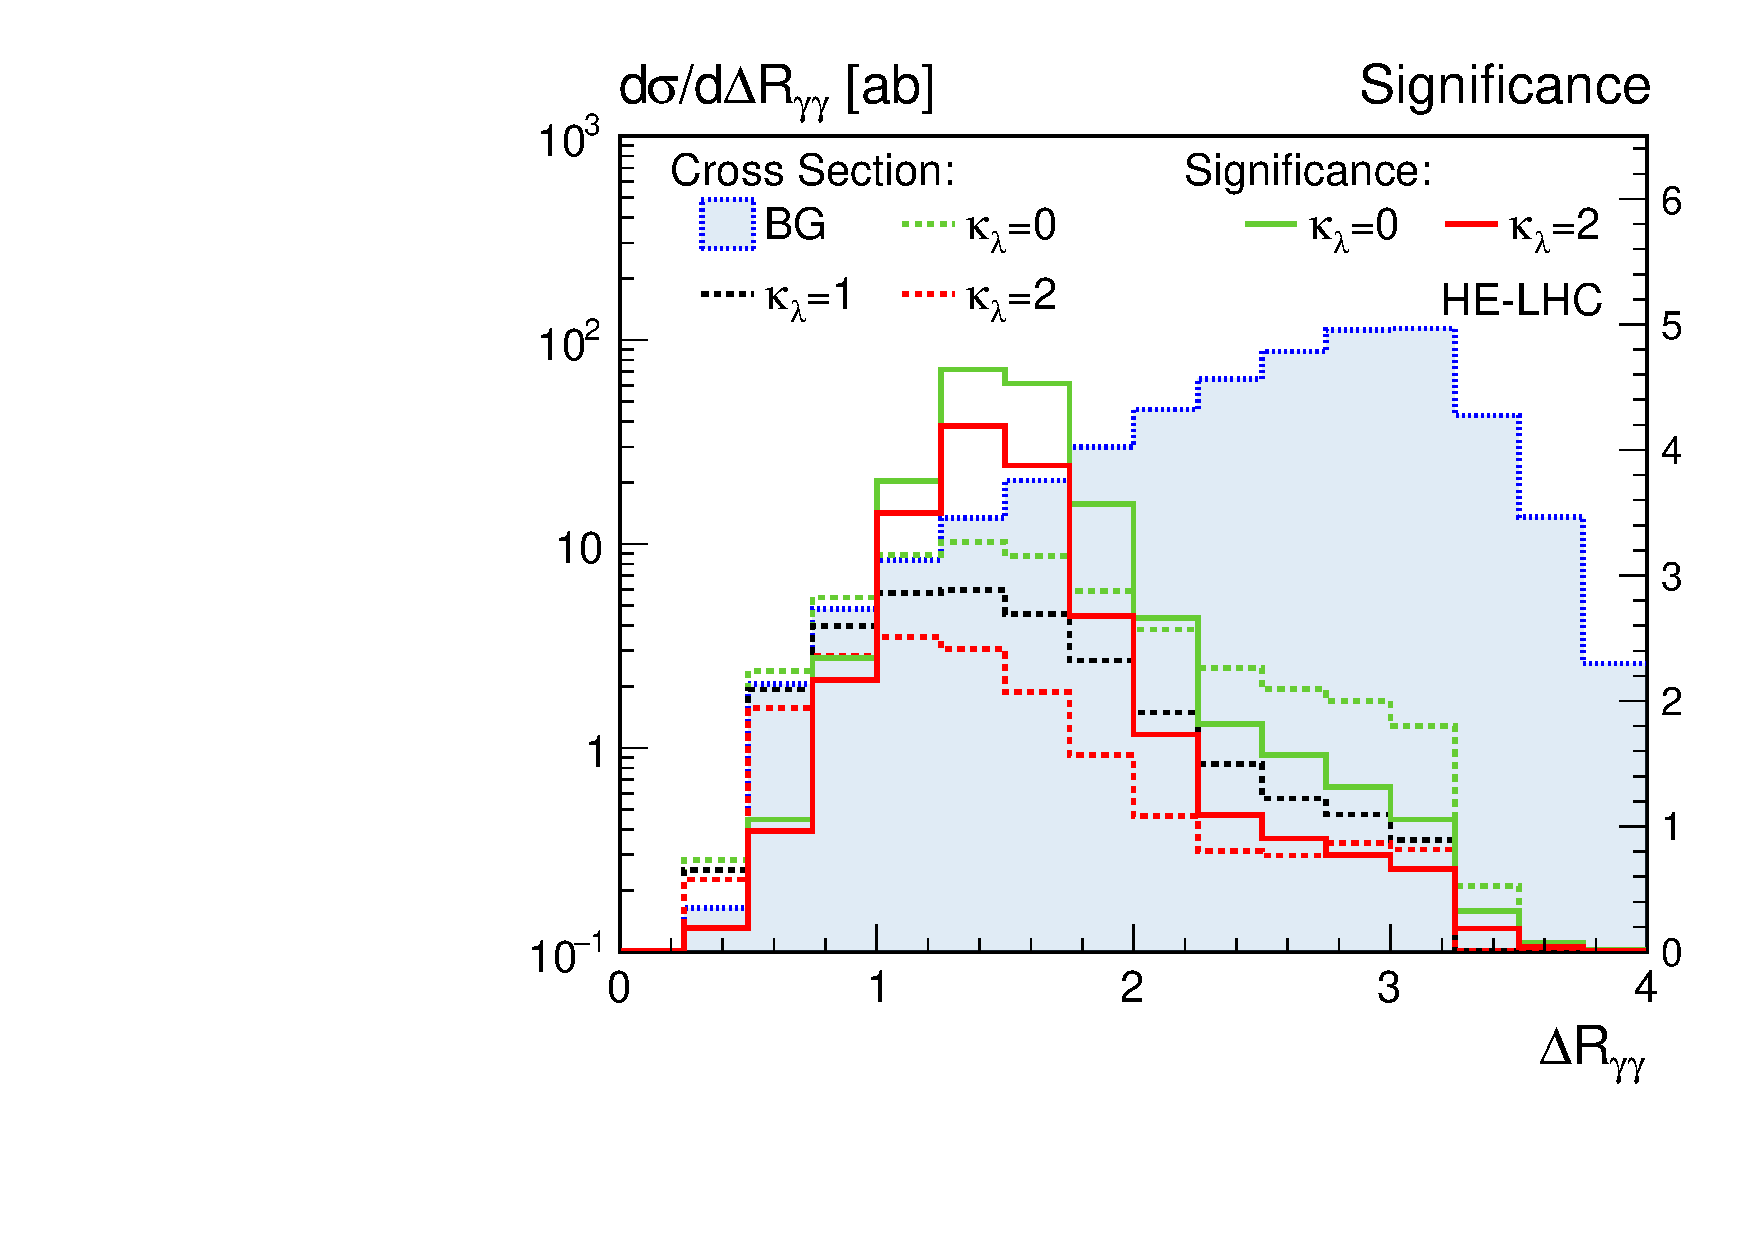
\includegraphics[width=0.32\textwidth]{\main/section3/plots/Plot_draa_27TeV}
  \caption{Kinematic distributions (dashed lines with left vertical
    axes) and significance distribution (solid lines with right
    vertical axes) assuming a Higgs self-coupling with
    $\kappa_\lambda=0,1,2$ for the HE-LHC. The significance describes the
    discrimination of an anomalous self-coupling $\kappa_\lambda \neq
    1$ from the SM hypothesis $\kappa_\lambda = 1$.}
\label{fig:madmax_diff}
\end{figure*}
%---------------------------------------------

%%%%%%%%%%%%%%%%%%%%%%%%%%
\asubsubsubsection{Detector-Level Analysis}

%-------------------------------------------------------
\begin{figure*}[b!]
\centering 
 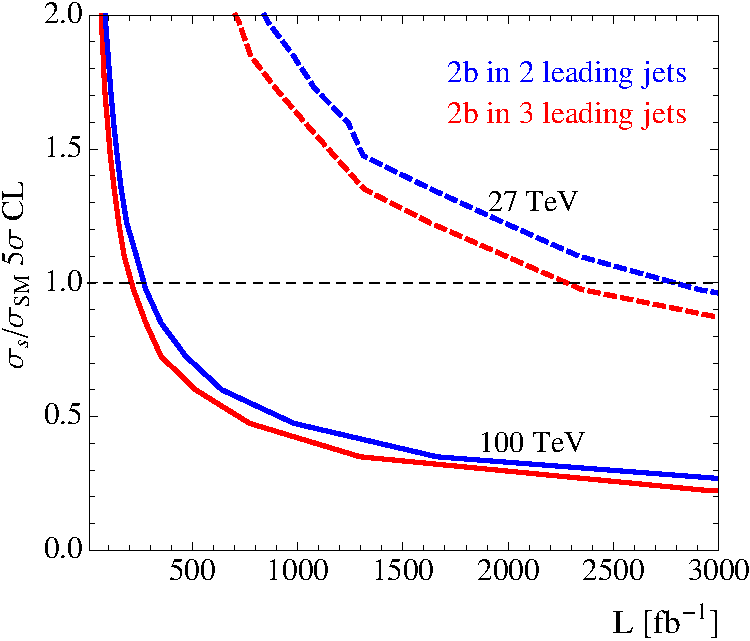
\includegraphics[width=.4\textwidth]{\main/section3/plots/hh_5sigma_2b3j} 
 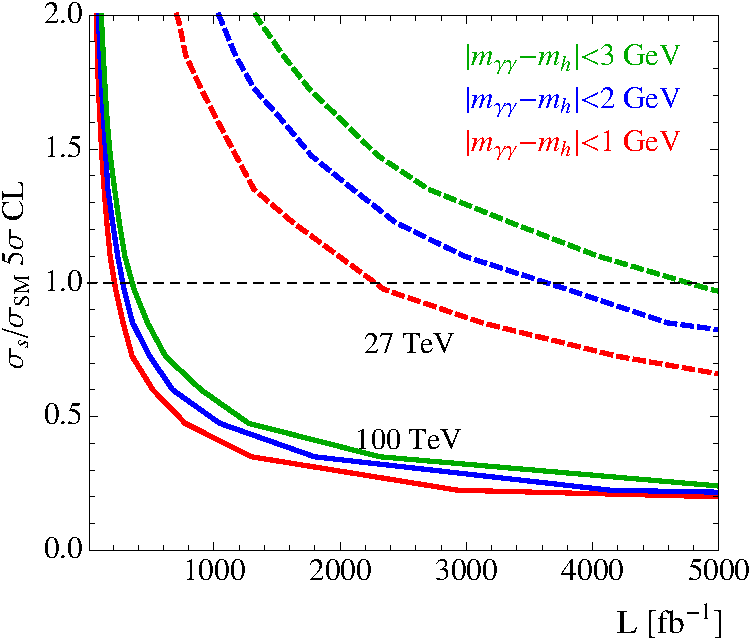
\includegraphics[width=.4\textwidth]{\main/section3/plots/hh_5sigma_width}
   \caption{Luminosity required for a $5\sigma$ discover of Higgs pair
     production for the HE-LHC (dashed) and a 100~\UTeV collider (full).
     Left: sensitivity in terms of the total rate, demanding two
     $b$-tags among the two or three leading jets and assuming
     $|m_{\gamma\gamma}-m_h|<1$~\UGeV.  Right: sensitivity for three
     mass windows $|m_{\gamma\gamma}-m_h|<1,2,3$~\UGeV.  We assume the
     SM hypothesis with $\kappa_\lambda=1$ and use a binned
     log-likelihood analysis of the $m_{hh}$ distribution.}
 \label{fig:bound1}
\end{figure*}
%-------------------------------------------------------

Based on our findings above, we now design a detailed analysis strategy to extract the Higgs
self-coupling with a focus on the shape of the $m_{hh}$
distribution~\cite{Goncalves:2018yva}. Our signal is $pp \to hh + X \to b\bar{b} \; \gamma \gamma + X$.
The signal and background samples are generated with
\textsc{MadGraph5}+\textsc{Pythia8}~\cite{Alwall:2011uj, Alwall:2014hca,Sjostrand:2007gs}, including one
extra jet using the \textsc{Mlm} scheme~\cite{Mangano2002}.\medskip

In the final state we demand two $b$-tagged jets and
two isolated photons with the minimal acceptance and trigger cuts
%
\begin{equation}
p_{T,j}>30~\GeV , \quad  
|\eta_j |<2.5, \quad 
p_{T,\gamma}>30~\GeV, \quad  
|\eta_\gamma| <2.5 , \quad 
\Delta R_{\gamma \gamma, \gamma j, jj} >0.4 \; .
\label{eq:base_selections}
\end{equation}
%
The background to our $b\bar{b} \; \gamma \gamma$ signal consists of
other Higgs production modes ($t\bar{t}h, Zh$) with $h \to \gamma
\gamma$, continuum $b\bar{b}\gamma\gamma$ production, and of multi-jet
events with light-flavor jets faking either photons or $b$-jets
($jj\gamma\gamma, b\bar{b}\gamma j$)~\cite{Baur:2003gp}.  

The proper simulation of efficiencies and fake rates are a key
ingredient for a realistic background estimate in this analysis.  For
the HE-LHC and the future 100~\UTeV collider we follow the ATLAS
projections~\cite{ATL-PHYS-PUB-2016-026}. The efficiency for a tight photon 
identification can be well parametrised by
%
\begin{align}
\epsilon_{\gamma\to\gamma} = 0.863 - 1.07 \cdot e^{-p_{T,\gamma}/34.8~\GeV}\;,
\end{align}
%
and a jet-to-photon mis-identification rate by
\begin{align}
\epsilon_{j\to\gamma} = 
\begin{cases} 
5.30\cdot 10^{-4}  \ \exp\big( -6.5 \left( p_{T,j}/(60.4~\GeV)- 1 \right)^2 \big) 
\quad &\text{ for } p_{T,j} <65~\GeV \;, \\
0.88 \cdot 10^{-4} \  \left[ \exp \big( -(p_{T,j}/(943~\GeV) \big) +248~\GeV/p_{T,j}\right]
\quad &\text{ for } p_{T,j} >65~\GeV \;.
%\;,
\end{cases}
\end{align}
%
This leads to a photon efficiency of about 40\% at $p_{T,\gamma}=30$~\UGeV,
saturating around 85\% for $p_{T,\gamma}>150$~\UGeV. Note that the 
Higgs decay products tend to be soft, $p_{T,\gamma}\sim m_h/2$. 
For $b$-tagging, we adopt an efficiency with $\epsilon_b =0.7$ associated 
with mis-tag rates of 15\% for charm quarks and 0.3\% for
light flavors. These flat rates present a conservative estimate from
the two dimensional distribution on $(p_{Tj},\eta_j)$ shown in the
HL-LHC projections~\cite{Kling:2016lay}. Encouragingly, the small light
flavor fake rate projections result in a strong suppression for the
initially dominant $jj\gamma\gamma$ background.

To control the continuum backgrounds, we require two Higgs mass windows,
%
\begin{align}
 |m_{bb}-m_h|<25~\GeV, \quad 
 |m_{\gamma\gamma}-m_h|<1~\GeV  .
 \label{eq:jreslov}
\end{align}
%
An obvious way to enhance the Higgs pair signal is to improve the
resolution on the reconstructed photons and $b$-jets from the Higgs
decays.  We adopt the rather conservative resolution for $m_{bb}$ as
in Eq.~\eqref{eq:jreslov}. Any improvement on it in experiments would
be greatly helpful for the signal identification and background
separation.  
\medskip

To take the information in the the differential distribution
$m_{hh}$ into account, we employ a binned log-likelihood analysis based on the 
CL$_{s}$ method, using the full $m_{hh}$ distribution to extract 
$\kappa_{\lambda}$~\cite{Read:2002hq}. As a starting point, we show the $5\sigma$ 
determination on the Higgs pair signal strength for the SM hypothesis $\kappa_{\lambda}=1$ as a 
function of the luminosity in the left panel of Fig.~\ref{fig:bound1}. Here 
we require two $b$-tagged jets among the two or three leading jets. We 
decompose the latter case in two  sub-samples $(bb,bbj)$ and $(jbb,bjb)$. 
We see how exploring the extra-jet emission significantly improves the 
significance as compared to the standard procedure adopted in the 
literature. The $5\sigma$ measurement for HE-LHC is pushed from 
$2.8~\iab$ to below $2.3~\iab$. 

In the right panel of Fig.~\ref{fig:bound1} we show the discovery reach for 
the Higgs pair signal at HE-LHC and a 100~\UTeV collider for three di-photon 
invariant mass resolutions described by a Gaussian width of 
$0.75,1.5,2.25$~GeV and corresponding Higgs mass windows 
$|m_{\gamma\gamma}-m_h|<1,2,3~\GeV$. As resolution of $1.5$~\UGeV 
has already been achieved at the LHC~\cite{CMS:2016zjv}. Higgs pair 
production will be discovered at the HE-LHC with approximately 
$2.5~...~5~\iab$ and at the 100~\UTeV collider with $0.2~...~0.3~\iab$ 
of data, in both cases well below the design luminosity.

%-------------------------------------------------------
\begin{figure}[t!]
\centering 
  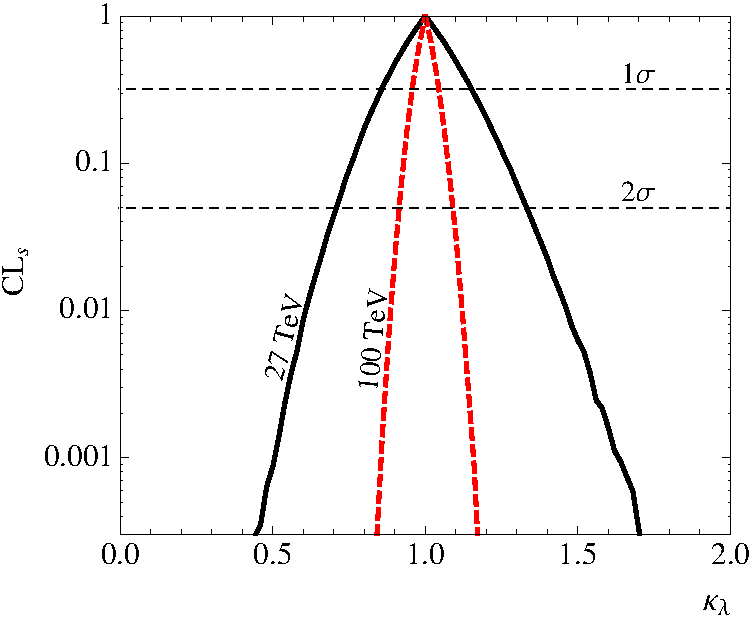
\includegraphics[width=.4\textwidth]{\main/section3/plots/hh_dlamb}
  \caption{Confidence level for separating an anomalous Higgs
    self-coupling hypothesis from the Standard Model
    $\kappa_{\lambda}=1$.}
 \label{fig:bound2}
\end{figure}
%-------------------------------------------------------

As commented in the introduction, there exist physics scenarios 
in which the Higgs self-coupling could be modified at the level of order 
one deviation from the SM value. The accurate measurement of the 
Higgs self-coupling via Higgs pair production at future colliders has the 
best promise to uncover the new physics associated with the Higgs sector.
In Fig.~\ref{fig:bound2}, we show the accuracy on this measurement. 
We find that the Higgs self-coupling can be measured with a precision
% 
\begin{align}
\kappa_{\lambda} &\approx 1 \pm 15\% \text{    at 68\% CL}\quad \text{and} \quad
\kappa_{\lambda} \approx 1 \pm 30\%   \text{    at 95\% CL}\quad\quad\quad
\text{(HE-LHC, 27~\UTeV, $15~\iab$)}  , \notag \\
\kappa_{\lambda} &\approx 1 \pm 5\% \;\; \text{    at 68\% CL}\quad \text{and}\quad
\kappa_{\lambda} \approx 1 \pm 10\% \text{    at 95\% CL} \quad\quad\quad
\text{(100~\UTeV, $30~\iab$).} 
\end{align}

While our conclusions on the determination of Higgs-self-interaction
at future hadron colliders are robust and important, there is still
room to improve. Although the final state $b\bar b\ \gamma\gamma$ is
believed to be the most sensitive channel because of the background
suppression and signal reconstruction, there exist complementary
channels such as ${gg\to hh \to b\bar b\ \tau^+\tau^-}$, $b\bar
b\ W^+W^-$, $b\bar b\ b\bar b$, etc. The kinematics-based measurement
and the all features related to QCD radiation at higher energies
should be equally applicable to all of them.

\begin{center}
\textit{by Samuel Homiller and Patrick Meade}
\end{center}

The Higgs self-coupling plays a central role in the spontaneous breaking of electroweak symmetry, and governs a pure elementary scalar interaction -- one that has never been observed in nature. Unfortunately, due to the small rate of $hh$ production, measuring the Higgs self-coupling at a $14\, {\rm \UTeV}$ appears exceedingly difficult unless it deviates substantially from the Standard Model value \cite{ATL-PHYS-PUB-2014-019, ATL-PHYS-PUB-2017-001}. A precision measurement of the Higgs self-coupling is thus one of the primary goals of any higher energy collider.  In this section we use the convention
\begin{equation}\label{eq:v_int}
  V_{\text{int}} = \lambda_3\frac{m_h^2}{2v}h^3 + \lambda_4\frac{m_h^2}{8v^2}h^4
\end{equation}
such that in the SM $\lambda_3=1$.

While the prospects of a $100\, {\rm \UTeV}$ collider in measuring the self-coupling have been well studied \cite{Contino:2016spe}, relatively less attention has been paid to intermediate energy colliders such as HE-LHC. Previous studies indicate that the $hh\rightarrow b\bar{b}\gamma\gamma$ channel has the most promising signature at hadron colliders, and this is expected to be true at $27\, {\rm \UTeV}$ as well. However, the $b\bar{b}\gamma\gamma$ channel still suffers from significant backgrounds from particle mis-identification in the detector, making a dedicated detector study including these effects essential. Finally, as discussed below, single-Higgs production -- including through gluon-fusion -- is a significant background that must be properly understood to accurately project the capabilities of HE-LHC. In what follows, we present a projection of the capabilities of a HE-LHC to measure the self-coupling with these intricacies carefully considered.

\asubsubsubsection{Signal and Background Simulations}

The signal and background samples generated for this study are summarised in Table \ref{t.backgrounds}. We also show the cross sections of $14\, {\rm \UTeV}$ samples generated for validation with previous projections. 

The details of the signal and background simulations mimic those in Ref. \cite{Homiller:2018dgu}. 
The $pp \rightarrow hh \rightarrow b\bar{b}\gamma\gamma$ signal is simulated at leading order using {\sc\small MadGraph5\_aMC@NLO}\ \cite{Alwall:2014hca, Hirschi:2015iia} using the NNPDF2.3LO PDF set \cite{Ball:2014uwa} including all finite top mass effects. The {\sc\small MadSpin}\ package \cite{Artoisenet:2012st} was used for the Higgs boson decays and {\sc\small Pythia~8}\ \cite{Sjostrand:2014zea} for the showering and hadronisation of events. The LO signal is normalised to match the state of the art NNLO/NNLL calculation with finite top mass effects included at NLO in QCD~\cite{Grazzini:2018bsd}. Additional samples with the self-coupling modified to values between $-1$ and $10$ times the SM value were also generated. Representative kinematic distributions of the signal at parton level are shown in Fig. \ref{fig:dihiggs_kinematics}.

\begin{figure}[h]
\centering
%\begin{subfigure}{.3\textwidth}
%	\centering
	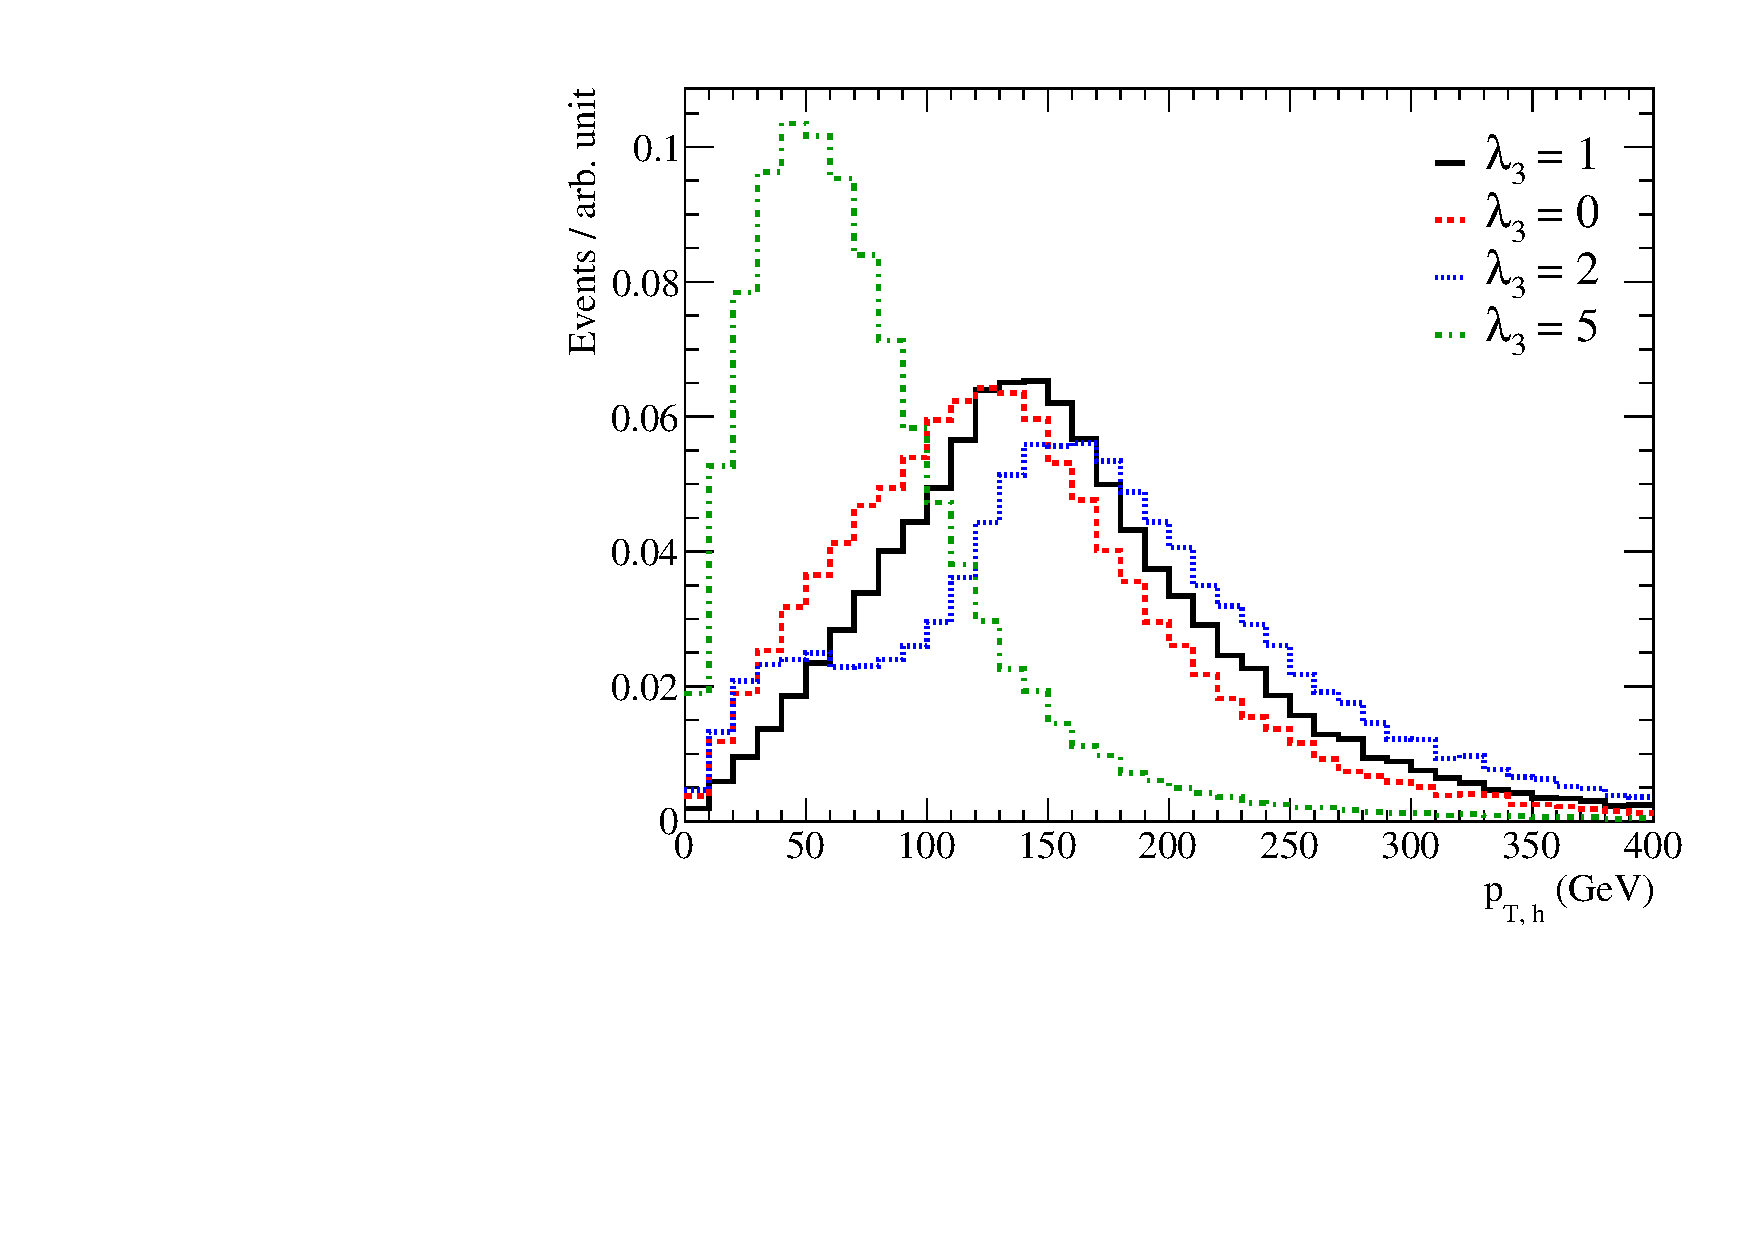
\includegraphics[width=0.32\linewidth]{\main/section3/plots/Higgs_PT.pdf}
	\hfill
%	\caption{}\label{fig:dihiggs_kinematics1}
%\end{subfigure}
%\begin{subfigure}{.3\textwidth}
%	\centering
	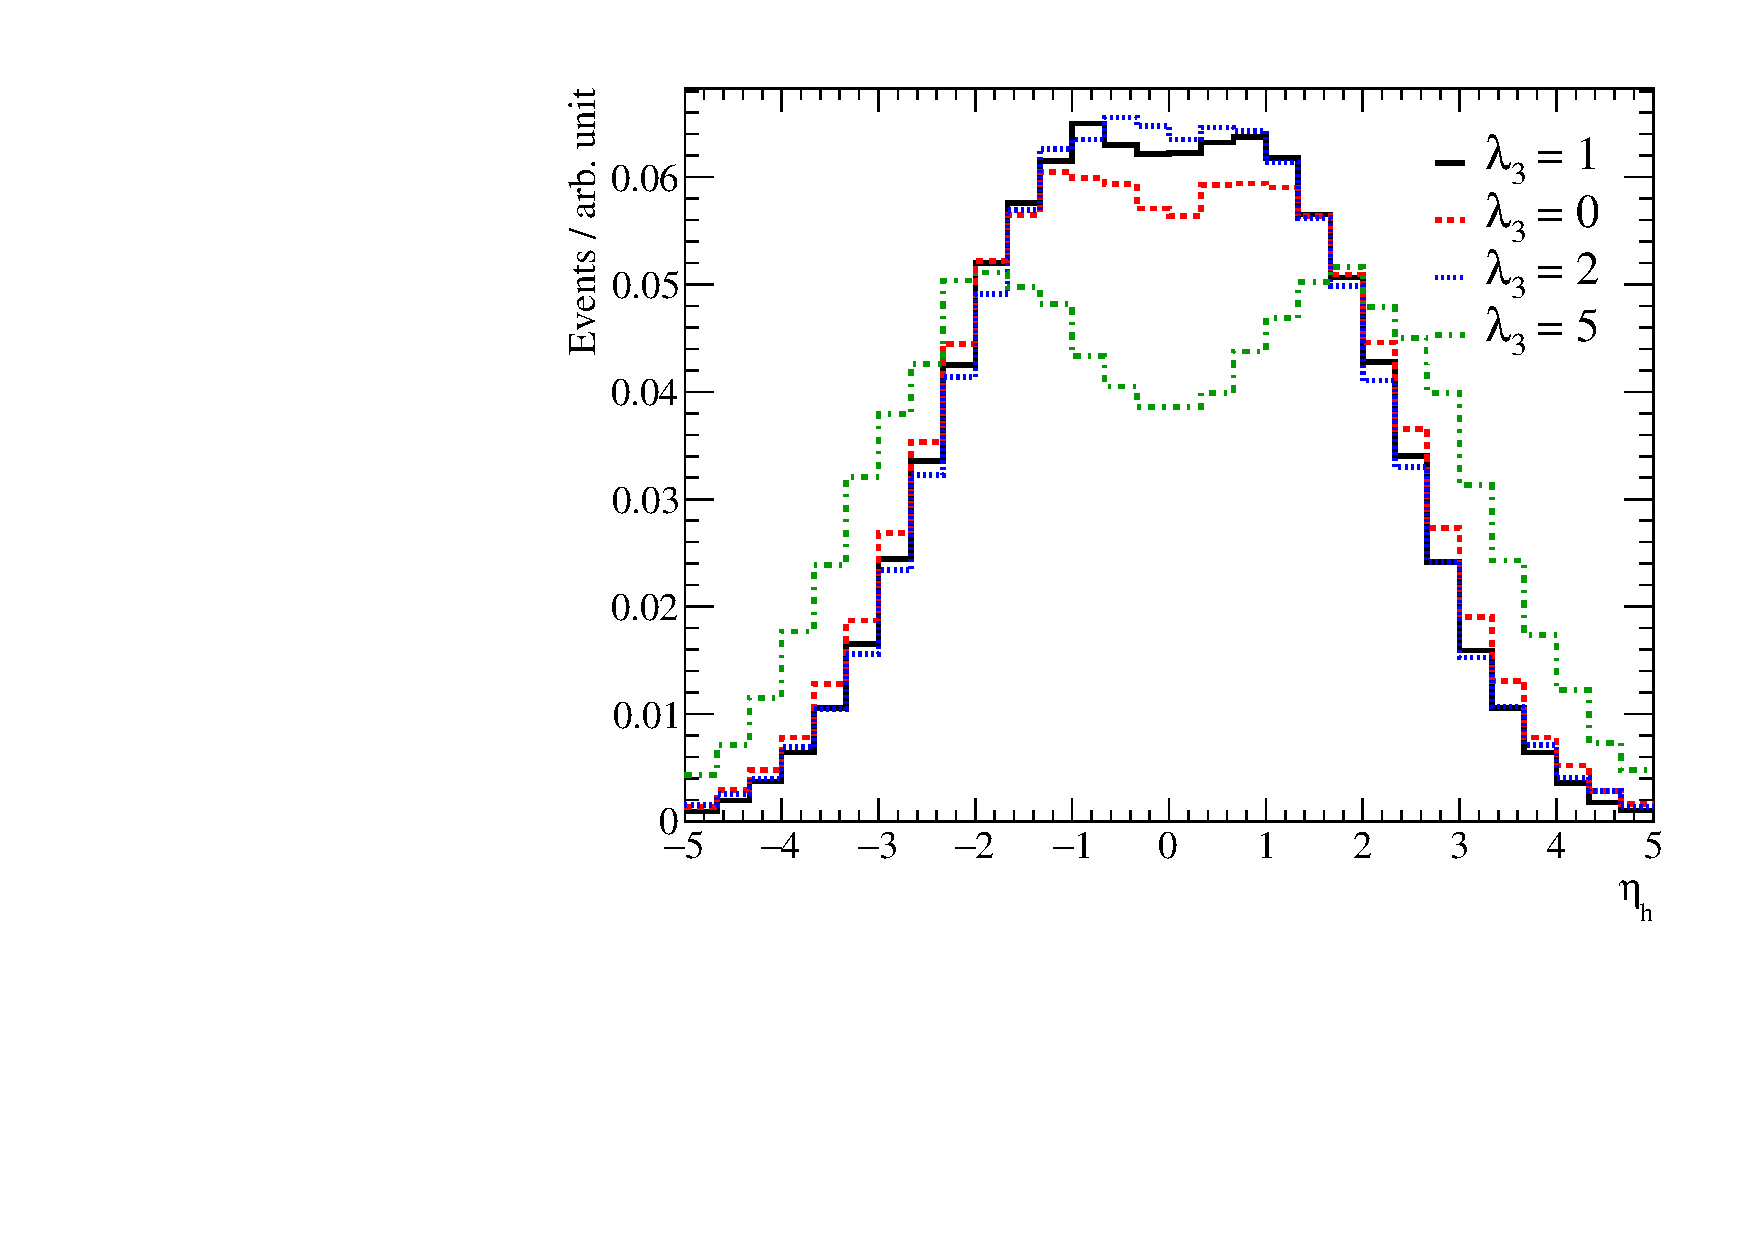
\includegraphics[width=0.32\linewidth]{\main/section3/plots/Higgs_Eta.pdf}
	\hfill
%	\caption{}\label{fig:dihiggs_kinematics2}
%\end{subfigure}%
%\begin{subfigure}{.3\textwidth}
%	\centering
	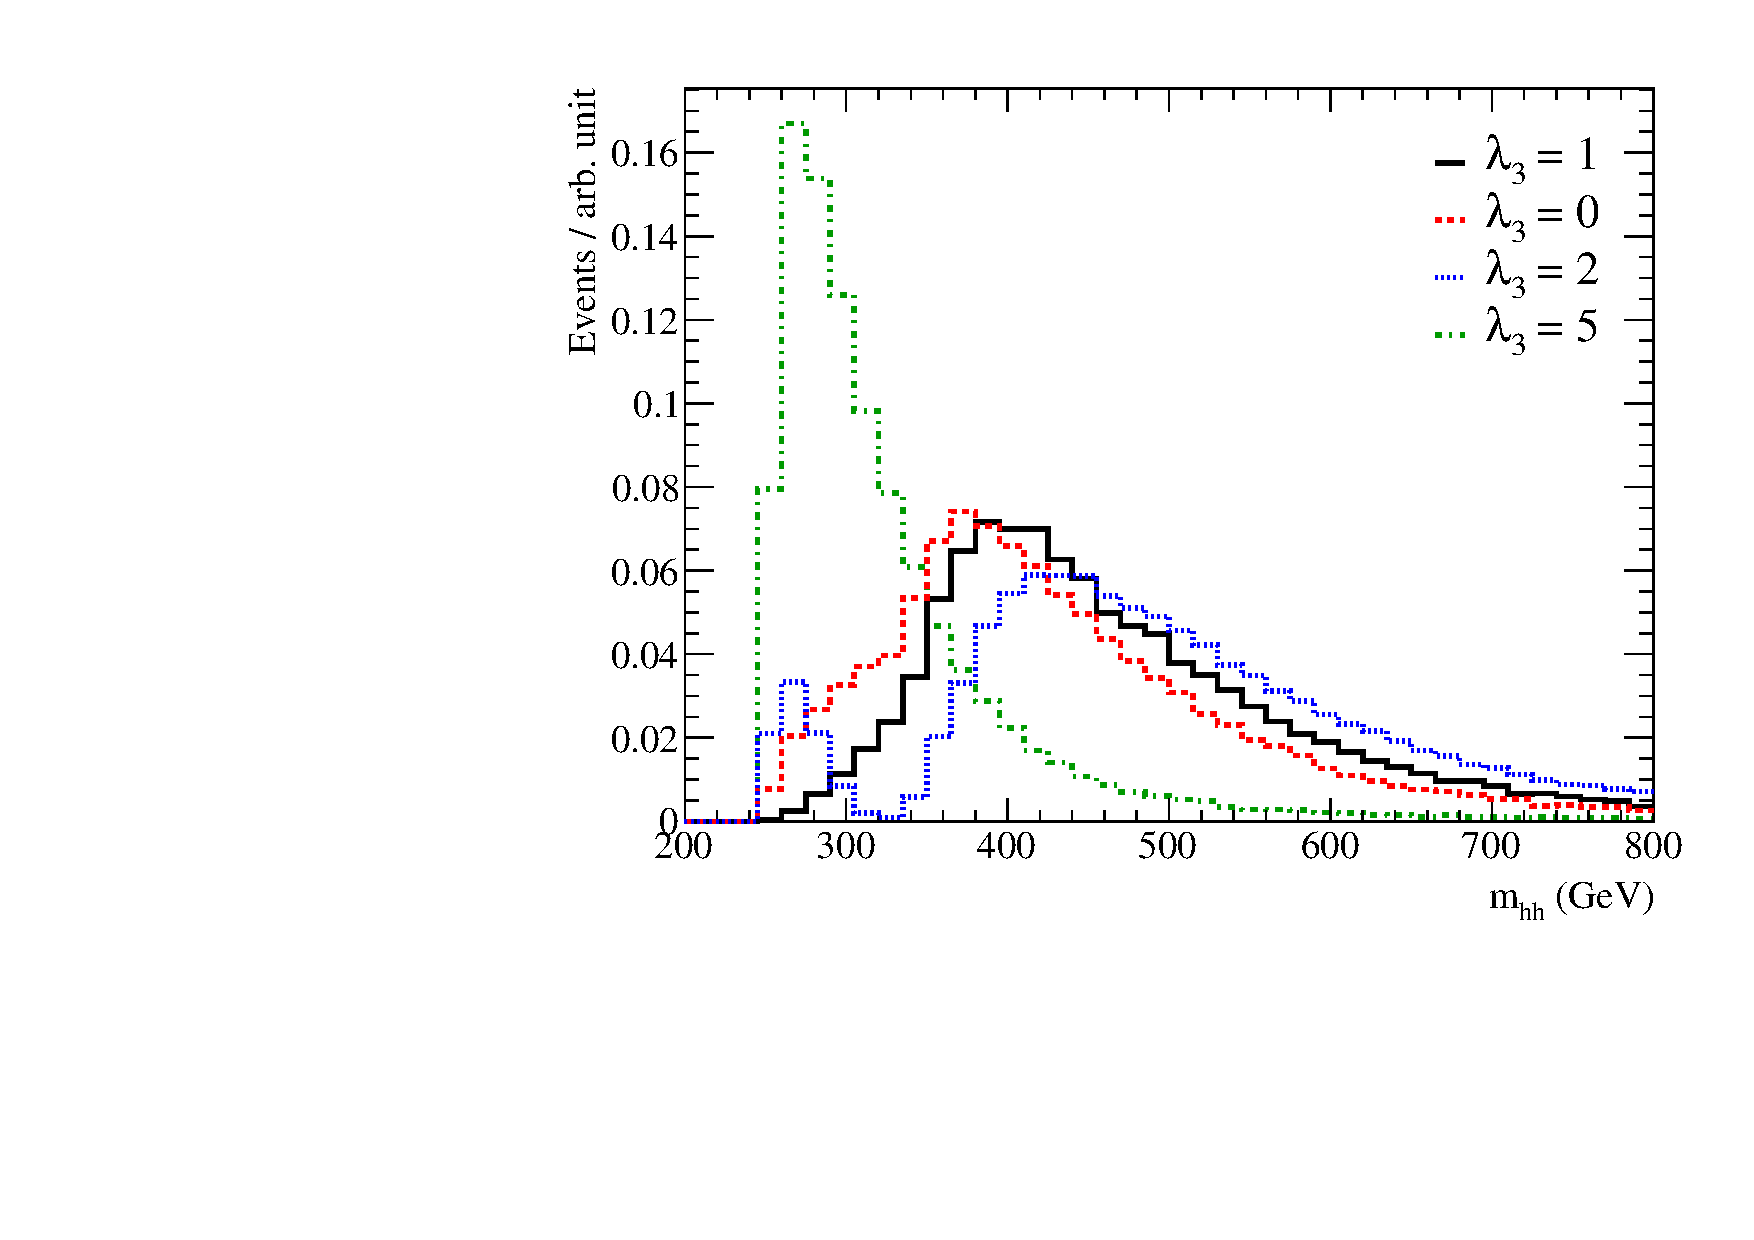
\includegraphics[width=0.32\linewidth]{\main/section3/plots/Higgs_Mhh.pdf}
%	\caption{}\label{fig:dihiggs_kinematics3}
%\end{subfigure}
\caption{(Left:) The transverse-momentum distribution of the true Higgs bosons generated in our 27 \UTeV samples, prior to showering and detector smearing, for several different values of $\lambda_3$. (Centre:) The same, but for the Higgs pseudorapidity. Right: The same, but for the distribution of the true Higgs pair invariant mass.}\label{fig:dihiggs_kinematics}
\end{figure}

Backgrounds to the $b\bar{b}\gamma\gamma$ decay channel include single Higgs production modes, non-resonant QCD backgrounds, as well as $Z(b\bar{b})\gamma\gamma$ and $t\bar{t}(+\gamma)$ production. We include all backgrounds where up to two additional photons or $b$-jets can arise from either misidentified light jets or electrons misidentified as photons.

The background from single Higgs production via gluon fusion ($ggF(\gamma\gamma)$) was generated in {\sc\small MadGraph}\ with up to two extra partons allowed in the matrix element, with no additional $k$-factor due to the already present real emissions. Events from other single Higgs production modes were generated directly in {\sc\small Pythia~8}\ at LO and normalised based on the recommendations in Ref. \cite{deFlorian:2016spz}. The remaining backgrounds were generated in {\sc\small MadGraph}\ interfaced with {\sc\small Pythia~8}\ for showering and hadronisation, with one additional jet allowed in the matrix element with MLM matching \cite{Mangano:2006rw, Alwall:2007fs} to the parton shower.

\begingroup
\renewcommand*{\arraystretch}{.7}
\begin{table}
\centering
\begin{tabular}{|c|c|cc|c|rcl|}
\hline
\multirow{2}{*}{Process}     & \multirow{2}{*}{Generator} & \multicolumn{2}{c|}{$\sigma \cdot BR$ {[}fb{]}} & \multirow{2}{*}{Order QCD} & \multicolumn{3}{c|}{Expected Events} \\
                              			&                   							& 14 \UTeV  			& 27 \UTeV  			&		& \multicolumn{3}{c|}{($27\, {\rm \UTeV}, 15~\text{ab}^{-1}$)} \\ \hline
$h(b\bar{b})h(\gamma\gamma)$  	& {\sc\small MadGraph}/{\sc\small Pythia~8} 	& 0.11      			& 0.41      			& NNLO/NNLL								& $209.6$		& $\pm$ & $0.2$ \\ \hline
$t\bar{t}h(\gamma\gamma)$     		& {\sc\small Pythia~8}           			& 1.40      			& 6.54      			& NLO  										& $286.8$		& $\pm$ & $1.6$\\
$Zh(\gamma\gamma)$            		& {\sc\small Pythia~8}           			& 2.24      			& 5.58      			& NLO 											& $67.1$ 		& $\pm$ & $0.7$ \\
%$b\bar{b}h(\gamma\gamma)$     	& {\sc\small Pythia~8}           			& 1.26      			& 3.42      			& NLO 											& $2.3$ 		& $\pm$ & $0.1$ \\
$ggF(\gamma\gamma)$           		& {\sc\small MadGraph}/{\sc\small Pythia~8} 	& 83.2      			& 335.1     		& $\text{N}^{3}\text{LO}$ 				& $349.7$ 	& $\pm$ & $9.5$ \\ \hline
$b\bar{b}\gamma\gamma$        	& {\sc\small MadGraph}/{\sc\small Pythia~8} 	& $3.4\times 10^{2}$     & $9.5\times 10^{2}$     & LO 					& $414.6$ 	& $\pm$ & $10.3$ \\
$c\bar{c}\gamma\gamma$        		& {\sc\small MadGraph}/{\sc\small Pythia~8} 	& $4.4\times 10^{2}$     & $1.5\times 10^{3}$     & LO 					& $185.7$ 	& $\pm$ & $4.2$ \\
$jj\gamma\gamma$              			& {\sc\small MadGraph}/{\sc\small Pythia~8} 	& $5.9\times 10^{3}$     & $1.4\times 10^{4}$     & LO 					& $63.3$ 		& $\pm$ & $3.8$ \\
$b\bar{b}j\gamma$             			& {\sc\small MadGraph}/{\sc\small Pythia~8} 	& $1.1\times 10^{6}$     & $3.4\times 10^{6}$     & LO 					& $199.6$ 	& $\pm$ & $9.4$ \\
$c\bar{c}j\gamma$             			& {\sc\small MadGraph}/{\sc\small Pythia~8} 	& $4.8\times 10^{5}$     	& $1.6\times 10^{6}$     & LO 				& $25.3$ 		& $\pm$ & $3.0$ \\
$b\bar{b}jj$                  					& {\sc\small MadGraph}/{\sc\small Pythia~8} 	& $3.7\times 10^{8}$     	& $1.5\times 10^{9}$     & LO 				& $155.4$ 	& $\pm$ & $8.2$ \\
$Z(b\bar{b})\gamma\gamma$   		& {\sc\small MadGraph}/{\sc\small Pythia~8} 	& 2.61     			& 5.23      			& LO 											& $21.5$ 		& $\pm$ & $0.4$ \\ \hline
$t\bar{t}$                    					& {\sc\small MadGraph}/{\sc\small Pythia~8} 	& $6.7\times 10^{5}$     	& $2.9\times 10^{6}$     	& NNLO 		& $11.6$ 		& $\pm$ & $3.3$ \\
$t\bar{t}\gamma$              				& {\sc\small MadGraph}/{\sc\small Pythia~8} 	& $1.7\times 10^{3}$     	& $7.9\times 10^{3}$     & NLO 				& $145.0$ 	& $\pm$ & $10.3$ \\ \hline
\multicolumn{5}{|c|}{Total Background}					& $1925.8$ & $\pm$ & $22.7$ \\ \hline
\multicolumn{5}{|c|}{Significance ($S/\sqrt{B}$)}		& $4.77$ & $\pm$ & $0.14$ \\ \hline
\end{tabular}
\caption{List of signal and background processes, the event generator used to simulate the matrix element and parton shower, and the cross section of each process along with the corresponding order in QCD at which the cross section is normalised. In the right-most column we show the expected number of events after all the event selection criteria have been applied.}
\label{t.backgrounds}
\end{table}
\endgroup

\asubsubsubsection{Detector Simulation}

To approximate the effects of detector resolution and reconstruction efficiencies, we use {\sc\small Delphes~3}\ with a dedicated card developed to approximate the performance of ATLAS and CMS at HL-LHC. We take this as a reasonable benchmark for the expected performance after the HE-LHC upgrade.

With respect to the {\sc\small Delphes}\ setup used in \cite{Homiller:2018dgu}, the card here has an improved E-Cal resolution and assumes a higher photon identification efficiency, but a somewhat degraded di-jet mass resolution. Aside from resolution and efficiency effects, particle mis-identification in the detector is also an important source of backgrounds to $hh\rightarrow b\bar{b}\gamma\gamma$. To avoid issues with MC statistics, we implement $b$-tagging and jet mis-tagging rates at analysis level using a reweighting scheme, with probabilities taken as functions of the jet $p_T$ as in Ref. \cite{Homiller:2018dgu}. These probabilities correspond to roughly $p_{b\rightarrow b} \approx 70\%$, $p_{c\rightarrow b} \approx 20\%$ and $p_{j\rightarrow b} \lesssim 1\%$. The probability for a light jet to fake a photon in the detector is also included via reweighting at analysis level as a function of $p_T$ (see \cite{Homiller:2018dgu}) which peaks at $5\times 10^{-4}$ for $p_{T,j} \sim 60\, {\rm \UGeV}$ before falling exponentially to $\sim 1\times 10^{-4}$.


\asubsubsubsection{Results and Limits on the Self-Coupling}

To isolate the $hh \rightarrow b\bar{b}\gamma\gamma$ signal, we implement selection cuts as follows:
\begin{itemize}
\setlength\itemsep{0.25em}
  \item At least 2 isolated photons and b-tagged jets with leading $p_T > 60\, {\rm \UGeV}$ and sub-leading $p_T > 35\, {\rm \UGeV}$, all with $|\eta_{\gamma,b}| < 2.5$.
  
\begin{minipage}{0.49\textwidth}
  \item $p_{T,\gamma\gamma}, p_{T,b\bar{b}} > 125\, {\rm \UGeV}$.
  \item $\Delta R_{b\bar{b}}, \Delta R_{\gamma\gamma} < 3.5.$
  \item $|m_{\gamma\gamma} - 125.0\, {\rm \UGeV}| < 4.0\, {\rm \UGeV}$.
  \item $|m_{b\bar{b}} - 125.0\, {\rm \UGeV}| < 25\, {\rm \UGeV}$.
\end{minipage}
\begin{minipage}{0.49\textwidth}
  \item $n_{\text{jets}} < 6$ for jets with $p_T > 30\, {\rm \UGeV}$, $|\eta| < 2.5$.
  \item No isolated leptons with $p_T > 25\, {\rm \UGeV}$.
  \item $|\cos\theta_{hh}| < 0.8$.
\end{minipage}
\end{itemize}

where $\cos\theta_{hh}$ is the decay angle of the Higgs boson pair evaluated in the lab frame (see Fig. \ref{fig:kinematics}).

\begin{figure}[ht]
\centering
%	\begin{subfigure}{0.49\textwidth}
%	\centering
	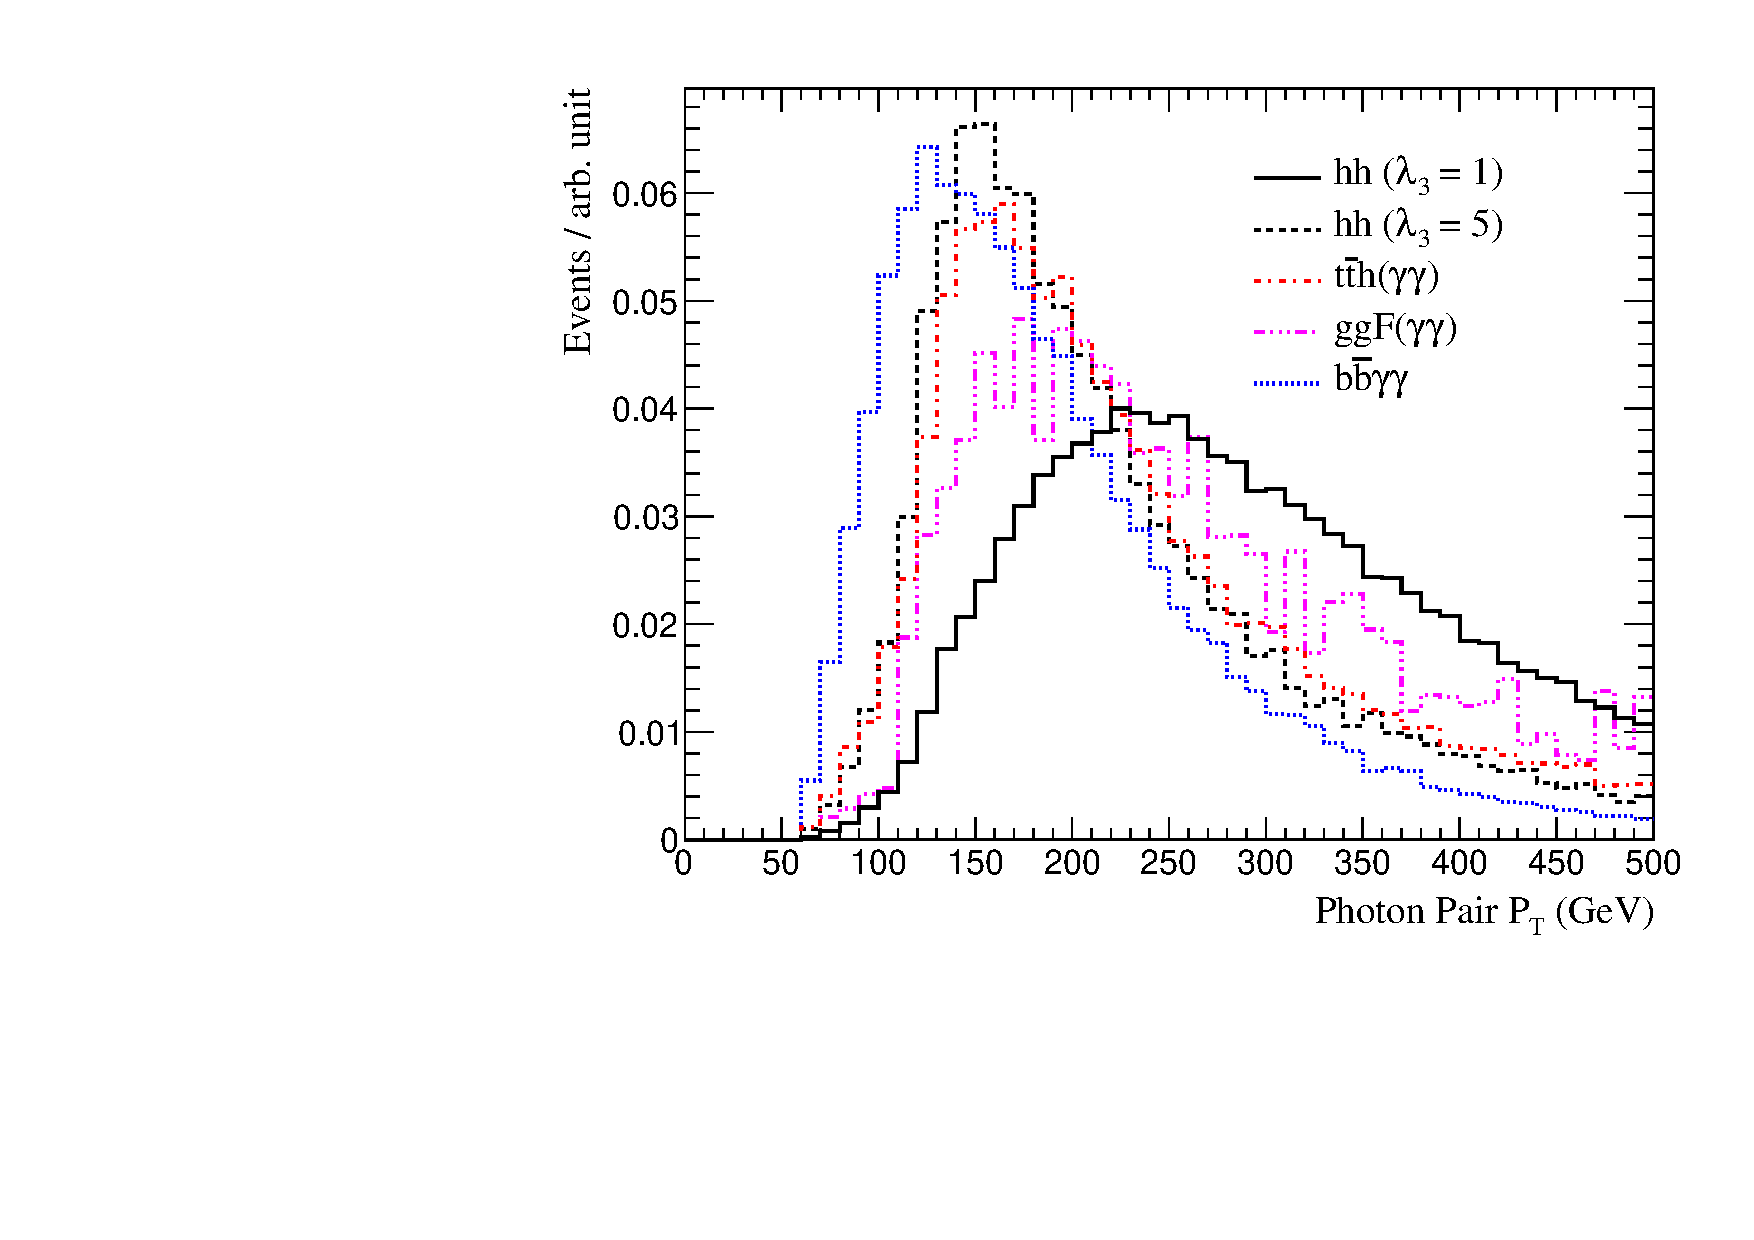
\includegraphics[width=0.49\linewidth]{\main/section3/plots/DiphotonPT}%\caption{}\label{fig:diphoton_pt}
%\end{subfigure}
\hfill
%\begin{subfigure}{0.49\textwidth}
%	\centering
	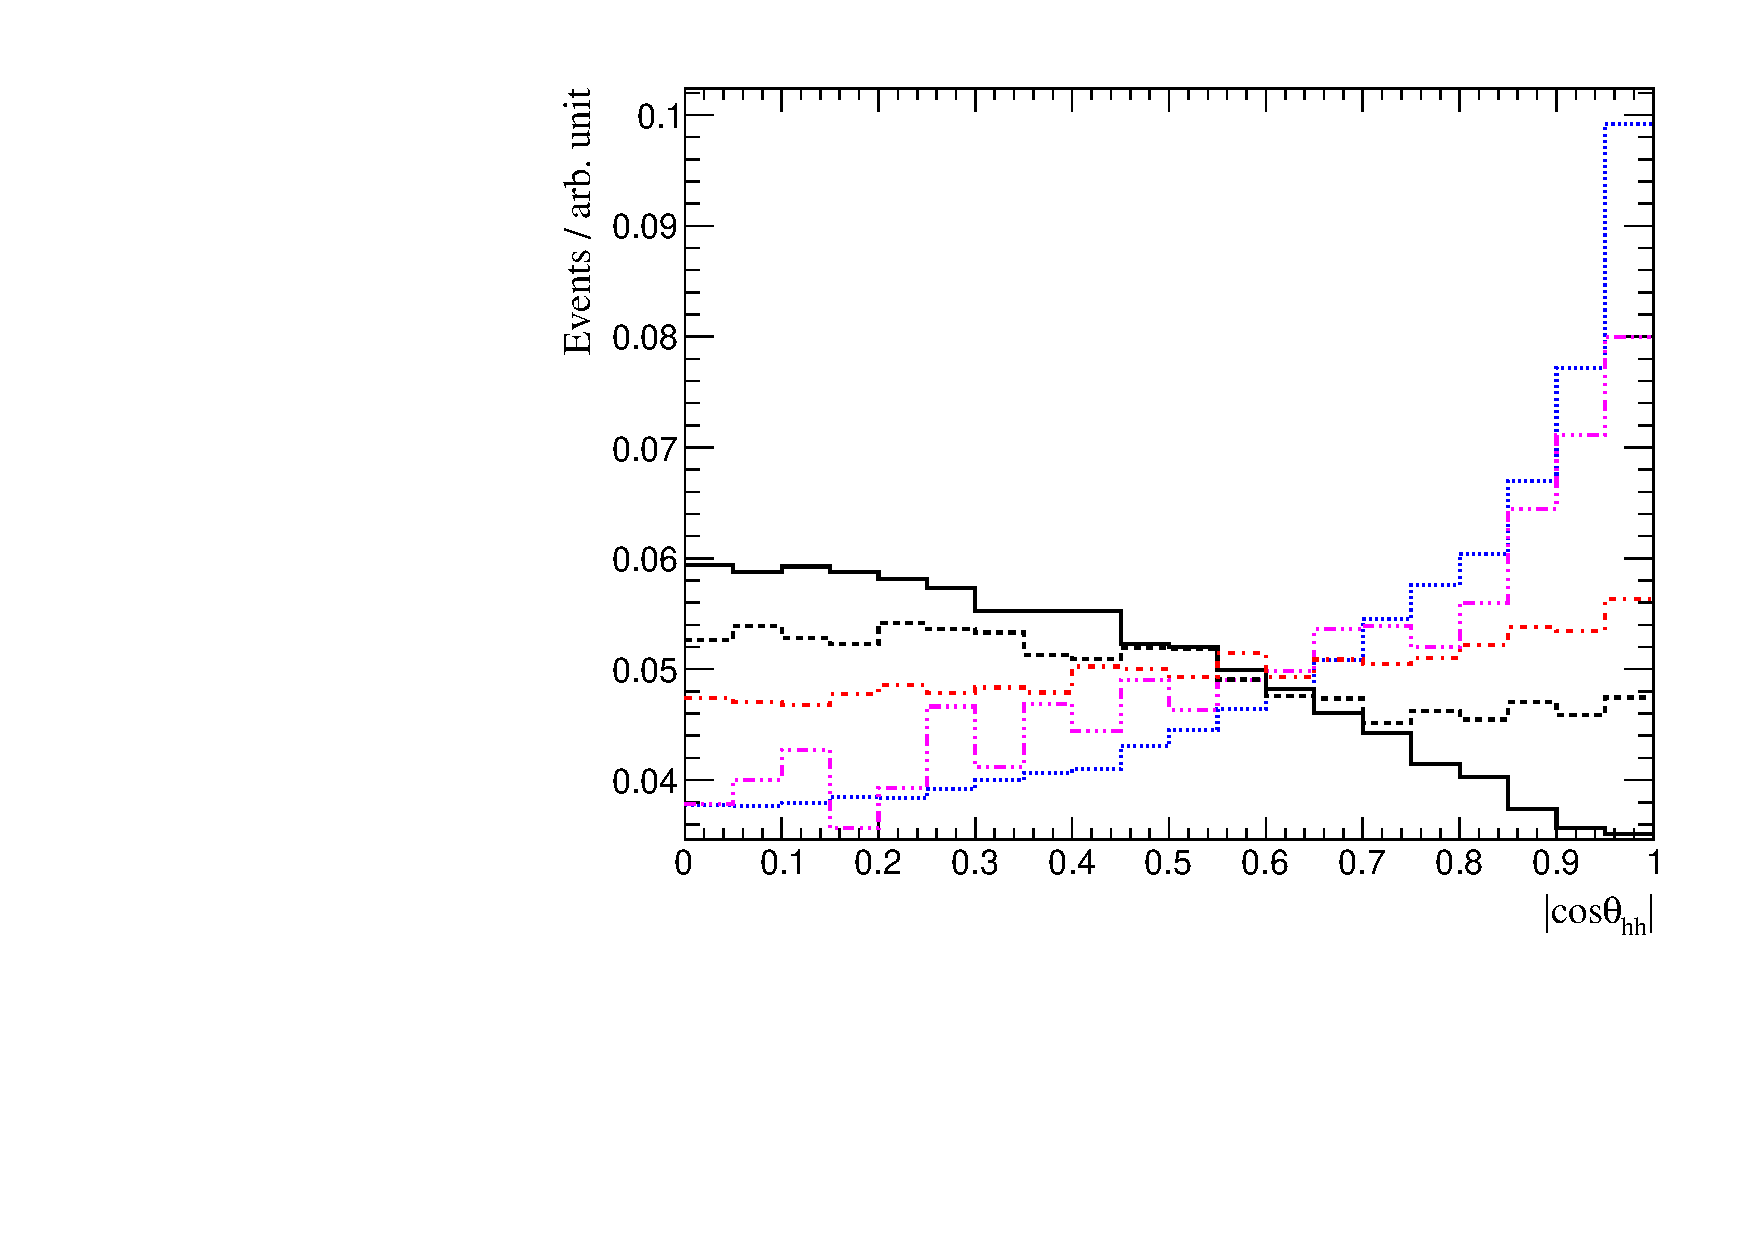
\includegraphics[width=0.49\linewidth]{\main/section3/plots/higgs_decayangle}%\caption{}\label{fig:decay_angle}
%\end{subfigure}
\caption{Normalised distributions of (Left:) the $p_T$ of the reconstructed $h\rightarrow\gamma\gamma$ and (Right:) the magnitude of $\cos\theta_{hh}$, the Higgs decay angle defined in the text. We show the distributions for the signal with $\lambda_{3} = 1$ and $5$ as well as several representative backgrounds.}
\label{fig:kinematics}
\end{figure}

Note that cuts on the $p_T$ and $\Delta_R$ of the $\gamma\gamma$ and $b\bar{b}$ pair are tightly correlated with the invariant mass of the $hh$ system. As seen in Fig. \ref{fig:kinematics} the photon pair $p_T$ has strong discriminating power for the SM $hh$ signal, but for non-SM values of $\lambda_{3}$, the signal and background become more degenerate.

The final selection efficiency is $3.4 \%$, and the expected number of events from each signal/background channel after applying all the cuts and detector effects is given in Table \ref{t.backgrounds} assuming $15~\text{ab}^{-1}$ integrated luminosity at HE-LHC. The uncertainty for each sample is estimated by partitioning the full event sample in to sub-samples and computing the standard deviation of the results from each sub-sample.

The largest backgrounds are from continuum $bb\gamma\gamma$ and single Higgs production and decay to $\gamma\gamma$. Particularly, we see that the $ggF$ induced mode contributes an $\mathcal{O}(1)$ background, despite being neglected in previous studies. The accurate modelling of the extra jets that arise in the hadron collision is a necessity for properly understanding this contribution.
Other large backgrounds arise from processes where a jet is reconstructed as a photon -- even when two fake photons are needed. Finally, we see that $t\bar{t}$ and $t\bar{t}\gamma$ are not insignificant backgrounds with the set of cuts we've applied. Several of these backgrounds might be mitigated by exploring the additional kinematic information in events with multiple jets, but the single-Higgs production backgrounds are difficult to reduce in light of the true $h\rightarrow \gamma\gamma$ present.

\begin{figure}
	\centering
	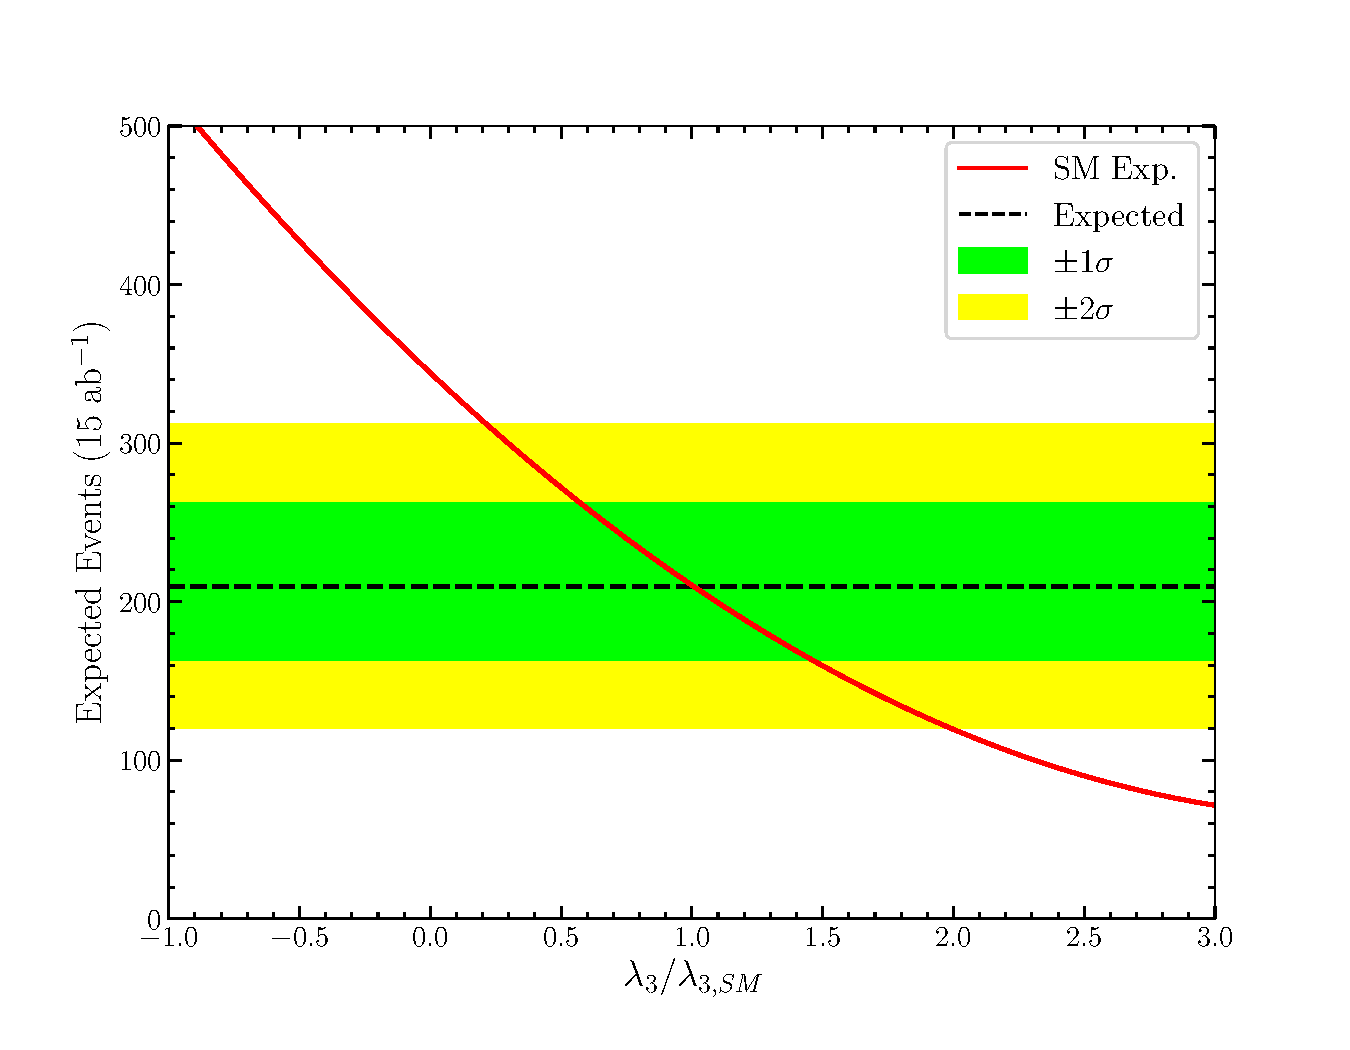
\includegraphics[width=8cm]{\main/section3/plots/lam3_limits_ylo}
	\caption{The expected number of signal events in a hypothetical experiment assuming the signal and background rates computed in Table \ref{t.backgrounds} at $L = 15~\text{ab}^{-1}$ for HE-LHC with the regular detector performance assumption. The black dashed line indicates the expected number of events from signal while the green (yellow) regions show the $1\sigma~(2\sigma)$ uncertainty regions arising from a likelihood scan with the statistical and MC uncertainties on the signal and background counts. The red curve shows the expected number of events from signal in a background free measurement as a function of $\lambda_3$, accounting for the changes in the signal acceptance due to kinematic differences at different $\lambda_3$}\label{fig:lam3_limit}
\end{figure}

To understand the attainable precision on $\lambda_{3}$, we assume a hypothetical observation of $S+B$ events after all selection cuts with $S$ and $B$ as in Table \ref{t.backgrounds}. This allows us to derive $68$ and $95\%$ confidence intervals on the expected number of signal events using a likelihood scan, including only the MC and statistical uncertainties. The expected number of signal events with $15~\text{ab}^{-1}$ integrated luminosity is plotted in Fig. \ref{fig:lam3_limit} along with the $1\sigma~(2\sigma)$ regions in green (yellow).

We can also compute the expected number of events at $15~\text{ab}^{-1}$ as a function of $\lambda_{3}$, taking into account both the varying $\sigma_{hh}$ cross section and the modified acceptance due to changes in the signal kinematics. The resulting curve is shown in red in Fig. \ref{fig:lam3_limit}. The intersection of this curve with the $1$ and $2\sigma$ regions indicate the expected precision on $\lambda_3$ in the absence of systematic uncertainties. We find

\begin{equation}
\lambda_{3} \in \left[ 0.58 ,  1.45 \right] \quad \text{at}~ 68\%~\text{C.L.}
\end{equation}

Note that, as a result of the destructive interference between the triangle and box diagrams leading to $hh$ production, there is a degeneracy in the expected number of events around $\lambda_3 \sim 5$. However, the kinematic structure of the $hh$ signal is very different at large values of $\lambda_3$, and such values could be easily rejected using differential measurements (e.g, with $m_{hh} = m_{b\bar{b}\gamma\gamma}$ or $p_{T,hh}$), so the degeneracy can be safely ignored for the purposes of this work.

In conclusion, we find that with a full account of the detector effects and backgrounds to $hh\rightarrow b\bar{b}\gamma\gamma$, a cut based analysis leads to an expected significance of $4.77 \pm 0.14 \sigma$, corresponding to a $45 \%$ measurement of the Higgs self-coupling at $27\, {\rm \UTeV}$ with $15~\text{ab}^{-1}$. Future improvements can be made both by considering other decay channels (e.g., $hh\rightarrow b\bar{b}b\bar{b}, b\bar{b}\tau\tau$, and $b\bar{b}WW$) and by exploiting the additional information present in the $hh$ invariant mass distribution, as discussed elsewhere in this report.

